\section{Tools and Applications}

The construction and analysis of CPN models have been supported by two
generations of graphical computer tools: Design/CPN and CPN
Tools. These tools have been instrumental to the success of CPNs as
they have enabled the application in a broad range of domains such as
distributed software systems, communication protocols, embedded
systems, and process- and worklow modelling. A comprehensive list
containing more than hundred modelling/analysis papers describing
practical applications and domains can be found via \cite{cpnuse}.

The first generation was the Design/CPN tool \cite{jensen:cpnmanual}
created at Meta Software, Cambridge, Massachusetts, USA starting in
1988 \cite{jensen:cpnmanual}. The main architects behind the tool were
Kurt Jensen, Robert Shapiro and Peter Hubert and the implementation
was made together with an international group of people including
Jawahar Malhotra (who got the idea to use the Standard ML language as
a basis for type definitions and net inscriptions), Ole Bach Andersen
(who implemented the graphical interface), S\o{}ren Christensen (who
implemented the complex algorithms for automatic binding of free
variables during simulations) and Hartmann Genrich (who contributed
with knowledge and experience from PrT nets). The first version of
Design/CPN supported modeling, syntax cheek and interactive
simulation. The introduction of hierarchical CPNs supported by the
Design/CPN tool made a dramatic change to the practical used of Petri
nets. The new modeling language and its tool support were general and
powerful enough to eliminate the need of making ad-hoc extensions as
discussed in the introduction of this paper. A common platform for
practical modeling had been established and this was used by most
Petri net practitioners. The use of the platform was supported by a
three volume monograph on Colored Petri Nets published by Kurt Jensen
in 1992-1997 \cite{jensen:cpnvols}. The CPN group at Aarhus University
was responsible for the development of the Design/CPN tool in the
period 1996-2002.

Starting from year 2000 a second generation of tool support, called
CPN Tools, was designed and implemented at Aarhus University,
Denmark. The main architects behind the new tool were Kurt Jensen,
S\o{}ren Christensen, and Michael Westergaard. The graphical user
interface was designed together with Michel Beaudouin-Lafon and Wendy
McKay from the international HCI research community. It is based on
empirical studies of the use of Design/CPN and much easier and
efficient to use. There is also a much faster simulation engine
(developed by Torben Haagh and Tommy Hansen). Many models run one
thousand times faster allowing complex automatic simulations to be
executed within seconds instead of hours. Many different kinds of
state space analysis are supported (developed by Lars Kristensen,
Michael Westergaard and Thomas Mailund). There is high-level support
for defining and collecting data from simulation-based performance
analysis (developed by Lisa Wells and Bo Lindstrøm). Finally there is
improved support for creating graphical feedback from ongoing
simulations (developed by Michael Westergaard).

CPN Tools supports the editing and construction of CPN models,
interactive and automatic simulation, state space-based model checking
(see sidebar), and simulation-based performance analysis (see
sidebar). Figure~\ref{fig:cpntools} provides a screenshot of CPN
Tools. The user of CPN Tools works directly with the graphical
representation of the CPN model. The graphical user interface (GUI) of
CPN Tools has no conventional menu bars and pull-down menus, but is
based on interaction techniques, such as \concept{tool palettes} and
\concept{marking menus}. The rectangular area to the left is an
\concept{index}. It includes the \figitem{Tool box}, which is
available for the user to manipulate the declarations and modules that
constitute the CPN model. The \figitem{Tool box} includes tools for
creating, copying, and cloning the basic elements of CP-nets. It also
contains a wide selection of tools to manipulate the graphical layout
and the appearance of the objects in the CPN model. The latter set of
tools is very important in order to be able to create readable and
graphically appealing CPN models. The remaining part of the screen is
the \concept{workspace}, which in this case contains four
\concept{binders} (the rectangular windows) and a circular pop-up
menu.

\begin{figure*}[b]
\centering
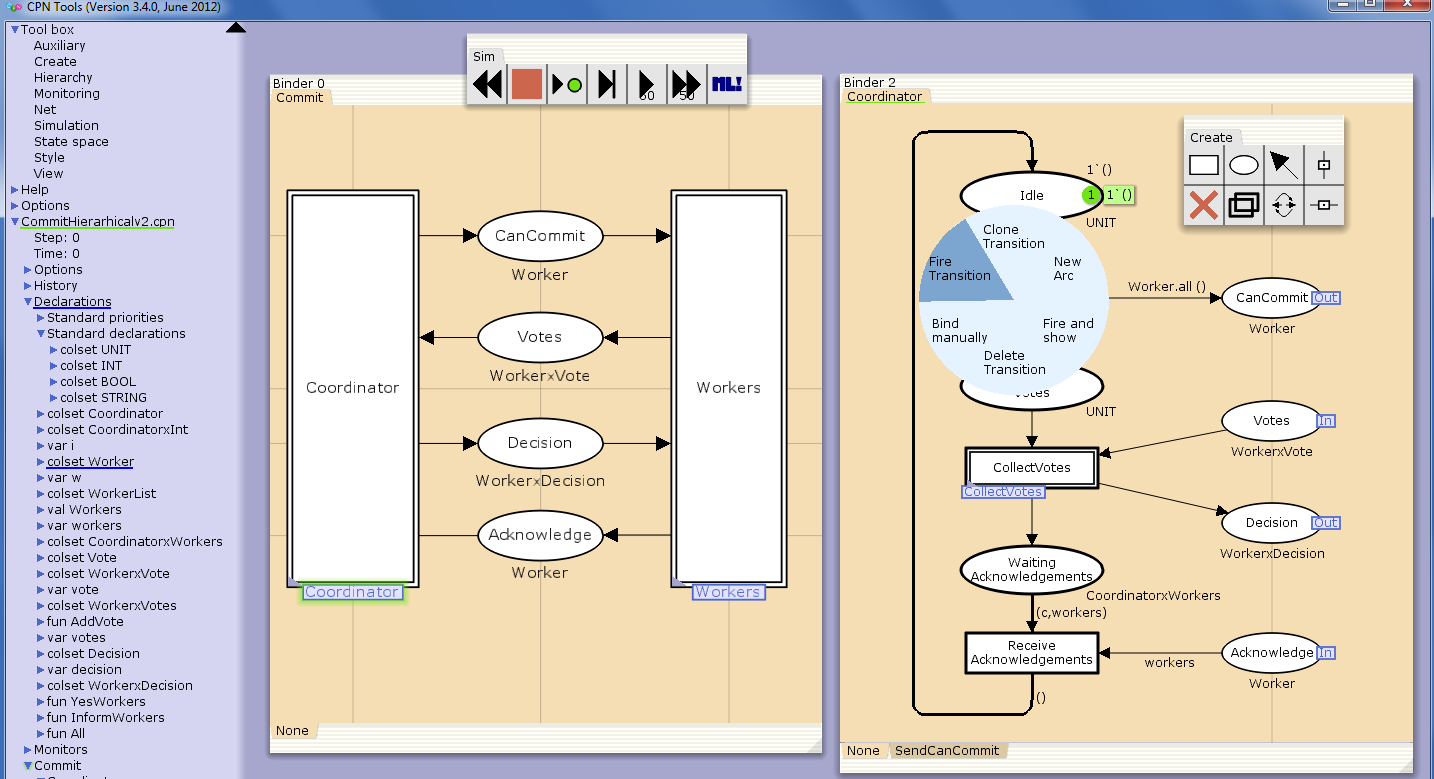
\includegraphics[width=\textwidth]{figures/cpntools.png}
\caption{Two-phase Commit Protocol in CPN Tools}
\label{fig:cpntools}
\end{figure*}

Each binder holds a number of items which can be accessed by clicking
the tabs at the top of the binder (only one item is visible at a
time). There are two kinds of binders. One kind contains the elements
of the CPN model, i.e., the modules and declarations. The other kind
contains the tools which the user applies to construct and manipulate
CPN models. The tools in a tool palette can be picked up with the
mouse cursor and applied. In the example shown, one binder contains
three modules named \figitem{Protocol}, \figitem{Sender}, and
\figitem{Receiver}, while another binder contains a single module,
named \figitem{Network}, together with the declaration of the colour
set \smlcode{NOxDATA}. The two remaining binders contain four
different tool palettes to \figitem{Create} elements, change their
\figitem{Style}, perform \figitem{Simulations}, and construct
\figitem{State spaces}.

Items can be dragged from the index to the binders, and from one
binder to another binder of the same kind. It is possible to position
the same item in two different binders, for example, to view a module
using two different zoom factors. A circular marking menu has been
popped up on top of the bottom left binder. Marking menus are
contextual menus that make it possible to select among the operations
possible on a given object. In the case of
Fig.~\ref{fig:cpntoolssnapshot}, the marking menu gives the operations
that can be performed on a port place object.

% syntax check and code generation

CPN Tools performs syntax and type checking, and error messages are
provided to the user in a contextual manner next to the object causing
the error. The syntax check and code generation are incremental and
are performed in parallel with editing. This means that it is possible
to execute parts of a CPN model even if the model is not complete, and
that when parts of a CPN model are modified, a syntax check and code
generation are performed only on the elements that depend on the parts
that were modified. 

% simulation

CPN Tools supports two types of simulation: interactive and
automatic. In an interactive simulation, the user is in complete
control and determines the individual steps in the simulation, by
selecting between the enabled events in the current state. CPN Tools
shows the effect of executing a selected step in the graphical
representation of the CPN model. In an automatic simulation the user
specifies the number of steps that are to be executed and/or sets a
number of stop criteria and breakpoints. The simulator then
automatically executes the model without user interaction by making
random choices between the enabled events in the states
encountered. Only the resulting state is shown in the GUI.  The
simulator of CPN Tools exploits a number of advanced data structures
for efficient simulation of large hierarchical CPN models. The
simulator exploits the locality property of Petri nets to ensure that
the number of steps executed per second in a simulation is independent
of the size of the CPN model. This guarantees that simulation scales
to large CPN models.

In 2010 CPN Tools had 10.000 licenses in 150 countries. At that time
the development and maintenance of the tool set were transferred to
the group of Wil van der Aalst at the Technical University of
Eindhoven, The Netherlands \cite{cpntoolsweb}. New updates with
improved functionality are made at a regular basis.  In addition, an
international standard for high-level Petri nets was developed and
approved in 2004 \cite{hcpnstandard}. The standardization work was
headed by Jonathan Billington and the standard is heavily based on
CPNs (which adhere to the standard).


